\documentclass{article}
\usepackage[utf8]{inputenc}
\usepackage{graphics}
\usepackage{kvmap}
%\usepackage{hyperref}


\title{\textbf {BCD TO EXCESS3 CONVERSION}}
\author{varsha reddy}

\begin{document}

\maketitle
\begin{tableofcontents}
\begin{abstract}
This manual shows how to convert a BCD numbers to Excess3 using seven segment display decoder to learn boolean logic.
\end{abstract}
\section{COMPONENTS}
\begin{tabular}{|c||c||c|}
\hline
\textbf{component} & {value} & {quantity} \\
\hline
 \textbf{Breadboard}  &  &  1  \\
 \hline
 \textbf{Resistor}  & {>=220ohm} & {1} \\
 \hline
 \textbf{Arduino} & {Uno} & 1\\
 \hline
 \textbf{Sevensegment display} & {common anode} & {1}\\
 \hline
 \textbf{Jumper wires} &   &  {20}\\
 \hline
\end{tabular}
\newline
\section{BCD TO EXCESS3 CONVERSION}
The excess-3 code (or XS3) is a non-weighted code used to express code used to express decimal numbers. It is a self-complementary binary coded decimal (BCD) code and numerical system which has biased representation. It is particularly significant for arithmetic operations as it overcomes shortcoming encountered while using 8421 BCD code to add two decimal digits whose sum exceeds 9. Excess-3 arithmetic uses different algorithm than normal non-biased BCD or binary positional number system.
\newline
\newline
\textbf{REPRESENTATION OF EXCESS-3 CODE}
\newline
\newline
Excess-3 codes are unweighted and can be obtained by adding 3 to each decimal digit then it can be represented by using 4 bit binary number for each digit. An Excess-3 equivalent of a given binary binary number is obtained using the following steps:
\newline
1. Find the decimal equivalent of the given binary number.
\newline
2. Add +3 to each digit of decimal number.
\newline
3. Convert the newly obtained decimal number back to binary number to get required excess-3 equivalent.
\newline
   You can add 0011 to each four-bit group in binary coded decimal number (BCD) to get desired excess-3 equivalent.
\newline
\newline
{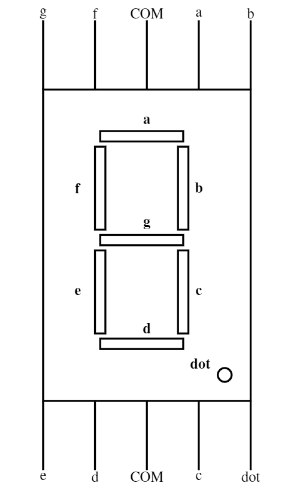
\includegraphics[scale=1]{7seg.png} } 

\newline
\newline
\textbf{KMAP FOR EQUATIONS}
\newline
\newline
\centering
\begin{kvmap}
\begin{kvmatrix}{C,D,A,B}
0&0&0&1 \\
0&1&0&1 \\
0&1&0&0 \\
0&1&0&0 \\
\end{kvmatrix}
\bundle[color=red]{3}{0}{3}{1}
\bundle[color=red]{1}{1}{1}{2}
\bundle[color=cyan]{1}{2}{1}{3}
\end{kvmap}
%\begin{equation}
\centering
\newline
W= AB'C'+A'BD+A'BC
%\end{equation}
\newline
\centering
\begin{kvmap}
\begin{kvmatrix}{C,D,A,B}
0&1&0&0 \\
1&0&0&1 \\
1&0&0&0 \\
1&0&0&0 \\
\end{kvmatrix}
\bundle[color=red]{0}{1}{0}{2}
\bundle[color=red]{0}{2}{0}{3}
\bundle[color=cyan]{1}{0}{1}{0}
\bundle[color=blue]{3}{1}{3}{1}
\end{kvmap}
\begin{equation}
X= A'B'D+A'B'C+A'BC'D'+AB'C'D
\end{equation}
\centering
\begin{kvmap}
\begin{kvmatrix}{C,D,A,B}
1&1&0&1 \\
0&0&0&0 \\
1&1&0&0 \\
0&0&0&0 \\
\end{kvmatrix}
\bundle[color=red]{0}{0}{1}{0}
\bundle[color=blue]{0}{2}{1}{2}
\bundle[color=cyan]{3}{0}{3}{0}
\end{kvmap}
\begin{equation}
Y=A'C'D'+A'C'D+AB'C'D'
\end{equation}
\centering
\begin{kvmap}
\begin{kvmatrix}{C,D,A,B}
1&1&0&1 \\
0&0&0&0 \\
0&0&0&0 \\
1&1&0&0 \\
\end{kvmatrix}
\bundle[color=red, invert=true,overlapmargins=8pt]{0}{0}{1}{3}
\bundle[color=cyan]{3}{0}{3}{0}
\end{kvmap}
\begin{equation}
Z= A'D'+AB'C'D'
\end{equation}
\newpage
\textbf{3. TRUTH TABLE}
\newline
\newline
\vspace{10mm}
\begin{tabular}{|c||c||c||c|}
\hline
\textbf{DECIMAL DIGIT} & {BCD CODE} & {EXCESS3} & {}\\
\hline
\textbf{}  & {A B C D}  & {W X Y Z} & {a b c d e f g}\\
\hline
\textbf{0} & {0  0  0 0} & {0  0  1 1} & {0 0 0 0 1 1 0}\\
\textbf{1} & {0  0  0 1} & {0  1  0 0} & {1 0 0 1 1 0 0}\\
\textbf{2} & {0  0  1 0} & {0  1  0 1} & {0 1 0 0 1 0 0}\\
\textbf{3} & {0  0  1 1} & {0  1  1 0} & {0 1 0 0 0 0 0}\\
\textbf{4} & {0  1  0 0} & {0  1  1 1} & {0 0 0 1 1 1 1}\\
\textbf{5} & {0  1  0 1} & {1  0  0 0} & {0 0 0 0 0 0 0}\\
\textbf{6} & {0  1  1 0} & {1  0  0 1} & {0 0 0 1 1 0 0}\\
\textbf{7} & {0  1  1 1} & {1  0  1 0} & {0 0 0 1 0 0 0}\\
\textbf{8} & {1  0  0 0} & {1  0  1 1} & {0 0 0 0 0 0 0}\\
\textbf{9} & {1  0  0 1} & {1  1  0 0} & {0 1 1 0 0 0 1}\\
\hline

\end{tabular}
\newline
\newline
5. Make connections according to the table\\
\newline
\begin{tabular}{|c||c||c||c||c||c||c||c|}
\hline
\textbf{Arduino} & 2 & 3 & 4 & 5 & 6 & 7 & 8\\
\hline
\textbf{display} & {a} & {b} & {c} & {d} & {e} & {f} & {g}\\
\hline
\end{tabular}
\newline
\end{tableofcontents}
\newline
\vspace{1cm}
\href{https://github.com/9705701645/Assignment1/tree/main/code/src}{https://github.com/9705701645/Assignment1/tree/main/code/src}
\end{document}